%!TEX root = ../memoire.tex

\chapter{GenDR: un réalisateur profond générique}\label{chapgendr}

GenDR (pour \emph{Generic Deep Realizer}) est un réalisateur profond multilingue \citep{lareau18} qui a hérité de l'architecture de MARQUIS \citep{WannerMARQUISGENERATIONUSERTAILORED2010} que nous avons présenté à la section \ref{sectionmarquis}. Comme son prédécesseur, GenDR est un transducteur de graphes basé sur la \ac{TST}, et ses dictionnaires et grammaires fonctionnent essentiellement de la même manière.

GenDR se démarque par sa capacité à traiter les collocations via les fonctions lexicales qui sont des concepts développés par la \ac{TST} pour expliquer comment se forment les collocations. Brièvement, la \ac{TST} a développé un mécanisme pour traiter les expressions comme \form{peur bleue} ou \form{grippe carabinée}. Dans ces deux cas, les modificateurs \sem{bleu} et \sem{carabiné} sont des intensificateurs qu'on représente par la fonction lexicale \lexfn{Magn}. Les fonctions lexicales modélisent les relations sémantico-lexicales entre ce type d'expression. Cela permet de rendre compte du fait que le lexème \lex{bleu} peut seulement agir en tant qu'intensificateur du lexème \lex{peur}. Dans d'autre cas, ça ne fait que signifier \sem{de couleur bleu}. Ainsi, c'est le lexème \lex{peur} qui sélectionne le lexème \lex{bleu} pour décrire un niveau d'intensité. On le représenterait ainsi \lexfn{Magn}(\lex{peur})=\lex{bleu}. Ce genre d'information doit être encodé dans un dictionnaire car ce ne sont pas des comportements prédictibles. Toutefois, il faut trouver un moyen d'encoder ce genre de phénomène dans un réalisateur si on souhaite générer du texte le plus naturel possible. Nous ne nous attarderons pas sur cette composante de GenDR puisqu'elle a été décrite dans un mémoire autre par \cite{LambreyImplementationcollocationspour2017}. \draft{est-ce que je devrais décrie les FL plus ou moins en détails ?}

Bref, GenDR offre une couverture beaucoup plus large que MARQUIS des fonctions lexicales en intégrant le module GÉCO \citep{lambrey15,LambreyImplementationcollocationspour2017}, qui implémente plus de 26\,000 fonctions lexicales (contre une trentaine pour MARQUIS). Toutefois, il est important de préciser que GenDR réalise en sortie des structures syntaxiques de surface. Le réalisateur se concentre principalement sur l'interface sémantique-syntaxe car c'est là qu'on peut modéliser les phénomènes langagiers profonds comme la lexicalisation et l'arborisation. Pour compléter la réalisation jusqu'au texte, il faut utiliser un réalisateur de surface qui prendrait les outputs de GenDR en entrée. D'ailleurs, \cite{MilleSharedTaskProposal2017a} ont mis au point un réalisateur de surface qui prend en input des arbres de dépendances universaux.

GenDR reprend les composantes de base de MARQUIS qui gèrent les phénomènes langagiers élémentaires comme la  lexicalisation simple, la complémentation et la modification. Ces règles forment le noyau du système et sont généralement partagées par l'ensemble des langues. Puis, les phénomènes grammaticaux spécifiques comme l'insertion des auxilaires ou des déterminants sont régis par des règles propres à chaque langue.

Le module sémantique contient 21 règles dont la plupart sont héritées de MARQUIS et 132 règles de lexicalisation \citep{LambreyImplementationcollocationspour2017}. Le module syntaxique contient nettement moins de règles. \draft{20 règles dont 12 partagées entre les langues.}\FL{pour les petits nombres, écris-les en français (vingt, douze)} Nous construirons donc la nouvelle version de GenDR à partir des bases de \cite{LambreyImplementationcollocationspour2017, lareau18,dubinskaite17}. Toutefois, nous avons retiré les fonctions lexicales de notre système car nous n'en avions pas besoin pour la nature de notre projet d'implémentation d'un dictionnaire verbal. Cela nous aurait demandé beaucoup de temps et ça n'aurai contribué en rien à la réussite (ou non) de l'implémentation.

%%%%%%%%%%%%%%%%%%%%%%%%%%%%%%%%%%%%%%%%%%%%%%%%%%%%%%%
% --------- A R C H I T E C T U R E  GENDR  ---
%%%%%%%%%%%%%%%%%%%%%%%%%%%%%%%%%%%%%%%%%%%%%%%%%%%%%%%
\section{Architecture de GenDR}

Les composantes lexicales et grammaticales de GenDR sont prises en charge par le transducteur de graphes MATE \citep{BohnetDevelopmentEnvironmentMTTbased2000a,BOHNET10,bohnet07}. Donc pour mieux comprendre comment la réalisation se déroule dans GenDR, il faut d'abord présenter comment fonctionne MATE.

\subsection{MATE}
MATE a été conçu à la base pour implémenter la \ac{TST} dans le but réaliser du texte. Tous les niveaux de représentations (voir section \ref{sec:semsynt}) de la \ac{TST} correspondent à des graphes et la transduction de ceux-ci est assurée par des ensembles de règles modélisant chaque interface. En plus d'opérer la transduction de graphes, MATE a aussi été conçu pour tester, développer et maintenir une grammaire computationnelle ce qui nous permet de réaliser du texte tout en testant des fondements théoriques.

MATE comprend un éditeur de dictionnaires, un éditeur de graphes et un éditeur de grammaires. Les dictionnaires encodent les unités sémantiques et lexicales, alors que Les grammaires sont composées de règles modélisant le passage d'un niveau de représentation à une autre. L'éditeur de graphes permet de construire et de visualiser ceux-ci. Le système comprend aussi un module d'inspection permettant de voir le déroulement de l'application des règles. Cet outil s'avère très utile au développement d'une grammaire, puisqu'il permet de cerner à quel endroit la réalisation a coincé. Pour plus de détails, voir \cite{BohnetOpensourcegraph2010,LambreyImplementationcollocationspour2017, LambreyGECOv1User}.

Nous allons maintenant montrer brièvement à quoi ressemblent les éditeurs dictionnairiques, grammaticaux et graphiques.

%%%%%%%%%%%%%%%%%%%%%%%%%%%%%%%%%%%%%%%%%%%%%%%%%%%%%%%
% ---------D I C T I O N N A I R E  ------------------
%%%%%%%%%%%%%%%%%%%%%%%%%%%%%%%%%%%%%%%%%%%%%%%%%%%%%%%

\subsubsection{Dictionnaires}\label{sec:dictio}

Tel que nous l'avons mentionné, GenDR se sert de dictionnaire pour décrire le vocabulaire qui sera utilisé dans les textes. Il en utilise 3, un qui fait le pont entre les unités sémantiques et les unités lexicales, un qui décrit le comportement syntaxique des unités lexicale, et un qui décrit les fonctions lexicales. Nous excluerons le troisième dictionnaire de la discussion pour les raisons mentionnées précédemment.

Nous commencerons par décrire \textbf{le dictionnaire sémantique}, car c'est le premier dictionnaire qui est utilisé par le système lors du passage de la \ac{RSem} à la \ac{RSyntP}. Cette ressource décrit les lexicalisations possibles pour un sémantème donné. La figure~\ref{fig:semanticon} présente une entrée typique dans ce dictionnaire, qu'on appelle \emph{semanticon}, dans GenDR.Ce dictionnaire est une source importante de paraphrasage puisqu'une unité sémantique peut habituellement se réaliser de plus d'une manière. Par exemple, en anglais, le sens \sem{owe} peut se réaliser par les lexèmes \lex{owe} (un verbe) et \lex{debt} (un nom).

\begin{minipage}{\linewidth}
\begin{lstlisting}[language=Xml, caption=Échantillon du \emph{semanticon}, label=fig:semanticon]
owe { lex = owe
      lex = debt }
\end{lstlisting}
\end{minipage}

\textbf{Le dictionnaire lexical}, appelé \emph{lexicon}, contient de l'information détaillée à propos des lexies d'une langue donnée. Les entrées contiennent: \ac{DPOS}, \ac{SPOS}, la diathèse et les \acp{GP}(ces concepts sont clarifiés à la fin du chapitre, section~\ref{sec:gp}). \draft{expliquer rapidement la diathèse et le gp, puis pointer vers la dernière section pour plus d'information} D'ailleurs, comme nous le verrons dans la figure~\ref{fig:lexicon}, ces informations lexicales ne sont pas toujours explicitées dans l'entrée lexicale, dans ces cas, elles sont héritées de la classe par défaut qui leur est attribuée.

Si on se fie à la figure~\ref{fig:lexicon}, le verbe \lex{owe} ne semble contenir que des \acp{GP}, mais il hérite de plusieurs traits découlant de son appartenance à la classe par défaut: \texttt{verb\_dit}. Cela permet à \lex{owe} d'hériter de son \ac{GP}. Ce mécanisme fonctionne en amont, dans le sens où la classe \emph{verb\_dit} hérite des traits de la classe qui lui est associée: \emph{verb\_dt}, puis successivement, de \emph{verb}.

Ce mécanisme facilite grandement l'encodage des unités lexicales car on n'a qu'à associer chaque nouvelle entrée lexicale à la classe par défaut qui lui appartient. D'ailleurs ce concept ne se limite pas qu'aux verbes, chaque partie du discours possède une classe par défaut. Dans le cas où l'information n'est pas celle qui est encodée par défaut, on peut spécifier la modification dans l'entrée lexicale directement. On voit un exemple à la figure \ref{fig:lexicon}. On remarque que la lexie \lex{owe} permet deux \ac{DPOS} différentes en tant que contraintes du deuxième actant syntaxique qu'elle contrôle: \lstinline!gp={II={dpos=Num}}! et \lstinline!gp={II={dpos=N}}!. Elle permet ainsi la sélection d'un actant de type nominal ou numéral.

\begin{minipage}{\linewidth}
\begin{lstlisting}[language=Xml, caption = Échantillon du \emph{lexicon}, label=fig:lexicon]
predicate {
  gp = { 1 = I
         2 = II
         3 = III
         4 = IV
         5 = V
         6 = VI }
}
verb : predicate {
  dpos = V
  spos = verb
  gp = {
     I = {
        dpos = N
        rel = subjective
     }
  }
}
verb_dt : verb {                   // direct transitive
  gp = {
     II = {
        dpos = N
        rel = dir_objective

     }
  }
}
verb_dit : verb_dt {              // direct ditransitive
  gp = {
     III = {
        dpos = N
        rel = indir_objective
        prep = to  

     }
  }
}
[...]
owe : verb_dit {
  gp = { II = { dpos=Num } }
  gp = { II = { dpos=N } }
}
\end{lstlisting}
\end{minipage}

Les dictionnaires anglais et français de GenDR contiennent les 1\,500 lexèmes les plus courants de chaque langue. Les dictionnaires lituanien \citep{dubinskaite17} et persan contiennent respectivement $\sim$180 et $\sim$60 lexèmes, assez pour tester le système.

%%%%%%%%%%%%%%%%%%%%%%%%%%%%%%%%%%%%%%%%%%%%%%%%%%%%%%%
% ---------G R A M M A I R E  ------------------
%%%%%%%%%%%%%%%%%%%%%%%%%%%%%%%%%%%%%%%%%%%%%%%%%%%%%%%

\subsubsection{Grammaires}

La grammaire de GenDR est organisée autour de deux modules de règles, un modulant l'interface \ac{RSem}-\ac{RSyntP} et l'autre modulant \ac{RSyntP}-\ac{RSyntS}. 

Le module \ac{RSem}-\ac{RSyntP} s'occupe de faire l'arborisation (algorithme \emph{top-down}) et la lexicalisation {sélection des lexèmes pour représenter les sémantèmes} profonde de l'input. Ce module est divisé est trois groupes de règles: le c\oe{}ur partagée par toutes les langues, les fonctions lexicales et les règles spécifiques à chaque langue. Le second module s'occupe de l'arborisation et la lexicalisation de surface (ajout des mots fonctionnels et relations de surface), il est divisé en 2: les règles partagées par toutes les langues et les règles propres à chaque langue. Nous présenterons en détail les règles principales de ces deux modules dans les sections \ref{sec:arbo} et \ref{sec:exemple}. \draft{à retravailler}

La figure~\ref{fig:root} présente une règle du module sémantique-syntaxe profonde. Toutes les règles sont décrites dans ce format. D'abord, en haut, on a l'interface dans laquelle la règle opère, le nom de la règle et l'identifiant de son groupe. Dans la partie gauche (\emph{Leftside}) on retrouve les n\oe{}uds et arcs du graphes de départ, puis dans la partie droite (\emph{Rightside}) on retrouve le graphe créé sortie. Finalement, la partie du bas contient les conditions d'application de la règle donnée. Nous verrons en détails l'application concrète de la règle~\ref{fig:root} à la section~\ref{sec:arbo}. D'ailleurs, pour une meilleure compréhension de la création de règles, nous vous invitons à lire le manuel de GeCo \citep{LambreyGECOv1User}.

\begin{figure}[htb]
	\centering
	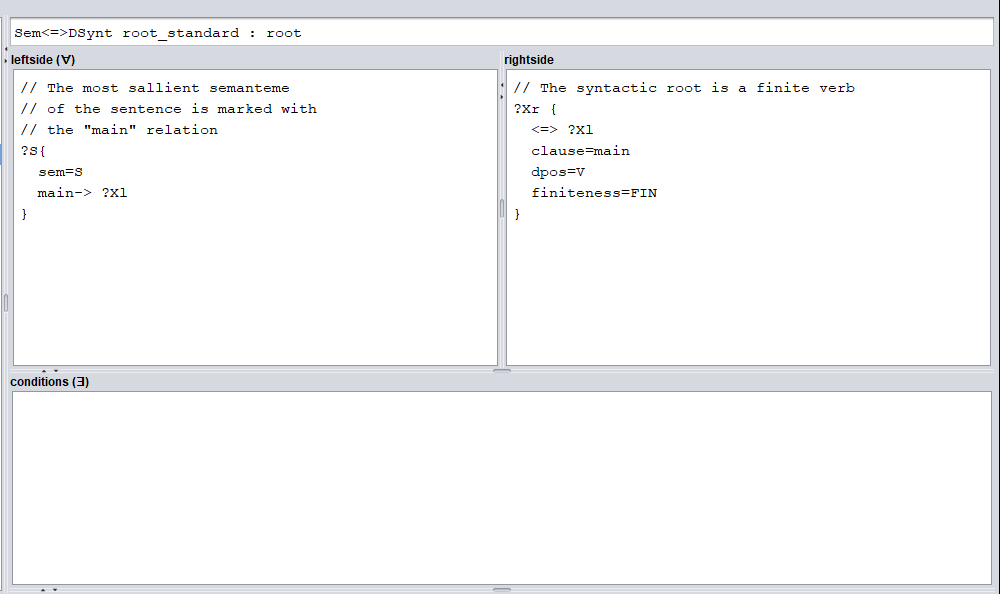
\includegraphics[width=1\textwidth, trim = {0cm 0cm 0cm 0cm},clip]{ch3/figs/grammaire.png}
	\caption{Règle créant la racine syntaxique}
	\label{fig:root}
\end{figure}

%%%%%%%%%%%%%%%%%%%%%%%%%%%%%%%%%%%%%%%%%%%%%%%%
% ---------G R A P H E S ------------------
%%%%%%%%%%%%%%%%%%%%%%%%%%%%%%%%%%%%%%%%%%%%%%%%

\subsubsection{Graphes}\label{entree-sortie}

Maitenant que nous avons fait un survol des dictionnaires et des modules de grammaires, il ne nous reste qu'à présenter les graphes. Dans un premier temps nous présenterons brièvement à quoi ressemble la construction d'un graphe en input. Puis nous montrerons à quoi ressemble les graphes en output.

L'input du réalisateur GenDR est un graphe sémantique \citep{mel2012semantics}\FL{\bf **** check ta biblio **** Daniel: le caractère spécial du c fonctionne pas avec Zotero, j'vais tenter de trouver une solution} où les prédicats sont liés à leurs arguments par des relations numérotées qui indiquent la position logique de l'argument. La figure~\ref{fig:debt} montre comment on construit un graphe sémantique dans MATE.

\begin{minipage}{\linewidth}
\begin{lstlisting}[language=XML, caption = Input sémantique, label=fig:debt]
structure Sem debt {
  S {
    owe {
    tense=PRES
    1-> Paul {class=proper_noun}
    2-> "\$500K" {class=amount}
    3-> bank {number=SG definiteness=DEF}}
    main-> owe } }
\end{lstlisting}
\end{minipage}

Toutefois, MATE offre aussi une version graphique pour encoder et visualiser le graphe sémantique (voir la figure \ref{fig:graphesem}).

\begin{figure}[htb]
	\centering
	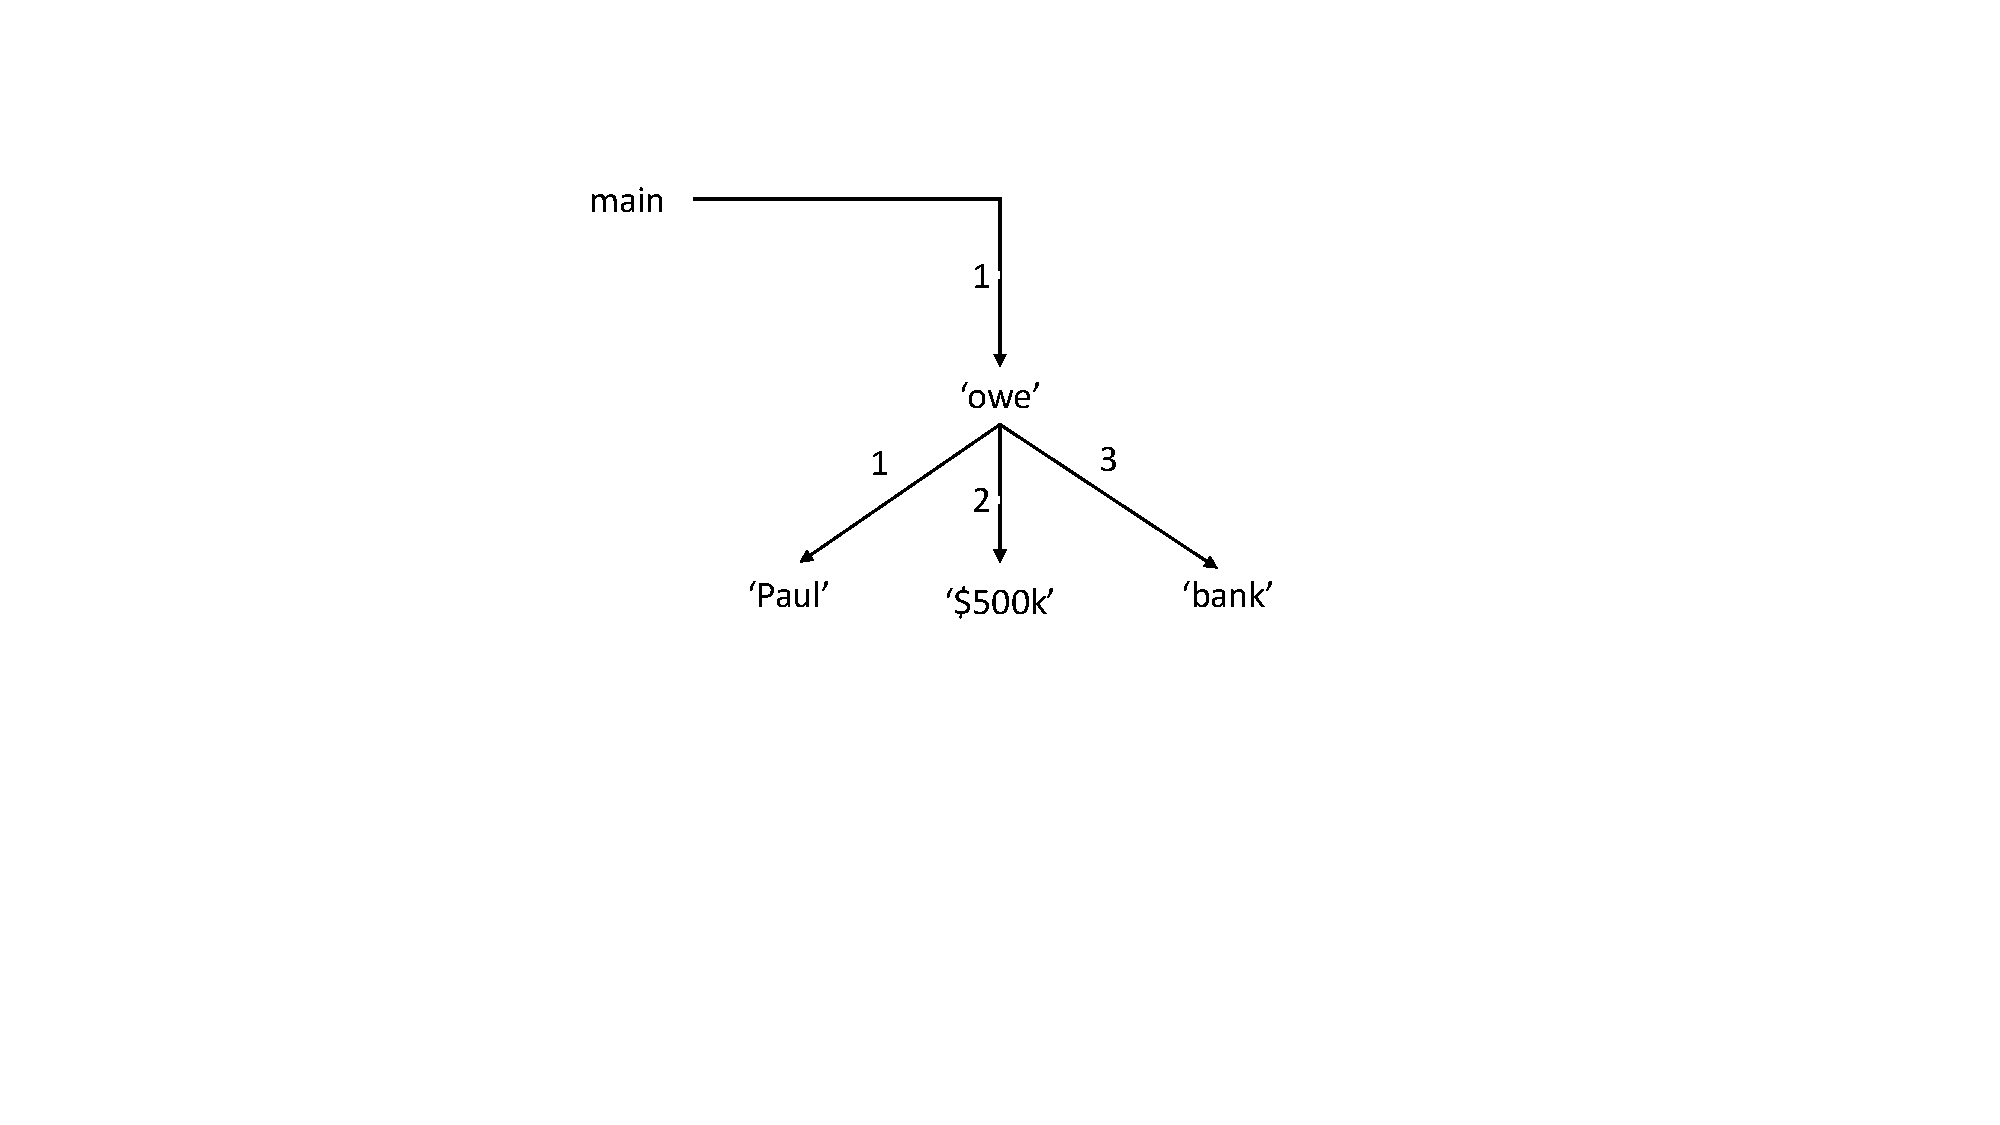
\includegraphics[width=1\textwidth, trim = {0cm 7cm 0cm 3cm},clip]{ch3/figs/owe_sem.pdf}
	\caption{Graphe sémantique en visuel}
	\label{fig:graphesem}
\end{figure}


La section graphe de GenDR nous permet de construire les structures sémantiques d'input et de visualiser les transductions de graphes. Pour l'input donné en \ref{input}, GenDR réalise six structures syntaxiques de surface. Celles-ci peuvent être visualisées dans MATE grâce au module de graphes. La figure \ref{fig:realsurfex} est un exemple d'output visuel que fournirait MATE. 

\begin{figure}[htb]
	\centering
	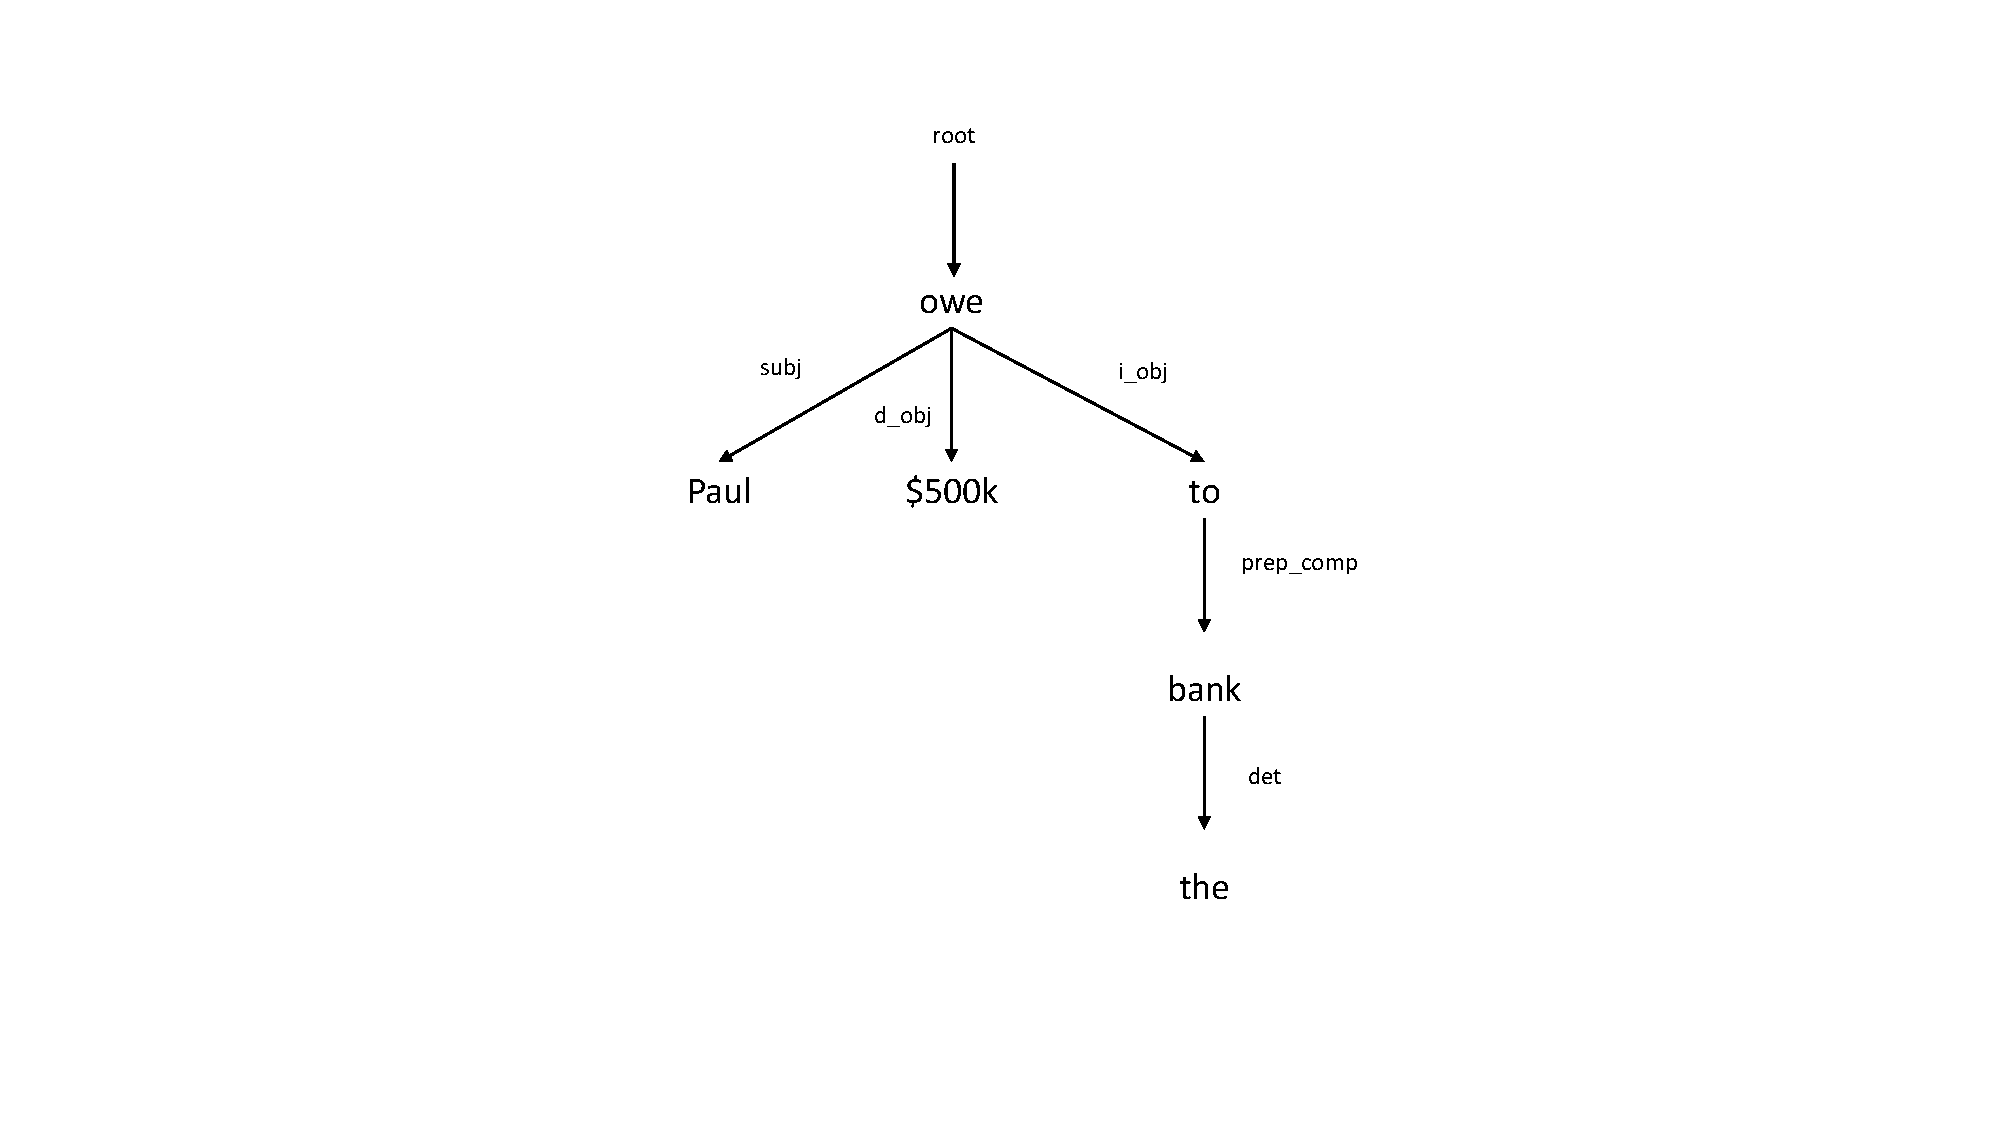
\includegraphics[width=1\textwidth, trim = {0cm 3cm 0cm 2cm},clip]{ch3/figs/realsurfex.pdf}
	\caption{Réalisation de surface}
	\label{fig:realsurfex}
\end{figure}

Toutefois, les modules de règles et de dictionnaires permettent en réalité de réaliser de six arbres syntaxiques superficiels (grâce aux mécanismes de paraphrasage). Nous les présentons à la figure \ref{fig:6realsurf}. Dans cette figure, les arbres de dépendances ont été linéarisés pour faciliter la compréhension du lecteur. Dans les faits, les arbres générés en output ne sont pas linéarisés et ils ressemblent à ceux de la figure \ref{fig:realsurfex}.

\begin{figure}[htb]
	\centering
	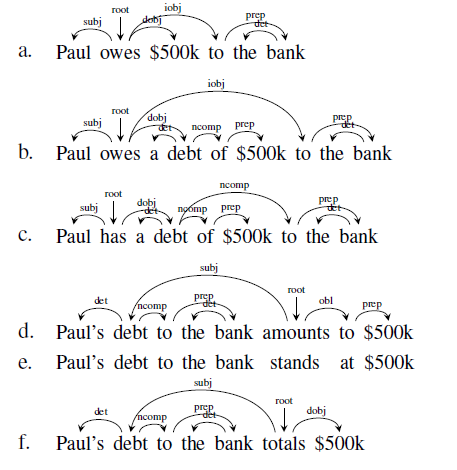
\includegraphics[width=0.5\textwidth, trim = {0cm 0cm 0cm 0cm},clip]{ch3/figs/exemples_real.png}
	\caption{Six réalisations syntaxiques de surface \citep{lareau18}}
	\label{fig:6realsurf}
\end{figure}
\FL{évite les captures d'écran si tu peux. Daniel: Oui, c'est temporaire, je vais tout' les refaire en pdf quand le texte sera prêt}

Si on souhaite une réalisation linéarisée et fléchie,  il faut utiliser un réalisateur de surface. C'est exactement dans ces contextes, que les réalisateurs de surface entrent en jeu \citep{DaoustJSREALTextRealizer2015, MolinsJSrealBBilingualText2015, GattSimpleNLGRealisationEngine2009, MilleSharedTaskProposal2017a,BelzFirstSurfaceRealisation2011}.

%%%%%%%%%%%%%%%%%%%%%%%%%%%%%%%%%%%%%%%%%%%%%%%%%%%%%%%%%%%%%%%%%%%%%%%%%%%%%
% --------- I N T E R F A C E   S É M A N T I Q U E- S Y N T A X E ---------
%%%%%%%%%%%%%%%%%%%%%%%%%%%%%%%%%%%%%%%%%%%%%%%%%%%%%%%%%%%%%%%%%%%%%%%%%%%%%

\section{Interface sémantique-syntaxe en TST}\label{sec:semsynt}

Dans la présente section, nous décrirons l'interface sémantique-syntaxe dans le cadre de la \ac{TST}. Plus précisément, nous expliquerons deux processus nécessaires au passage de la sémantique à la syntaxe: l'arborisation et la lexicalisation. Pour mieux comprendre où se situent ces procédés dans la modélisation du langage, nous ferons un très bref retour sur les fondements du cadre théorique que nous utilisons. 

La \ac{TST} vise la modélisation formelle de la correspondance entre les \emph{Sens} et les \emph{Textes} \citep{PolgueretheorieSensTexte1998, MelcukVerslinguistiqueSensTexte1997, DBLP:conf/coling/JolkovskyM67}. La figure \ref{fig:modeletst} (qui est issue de\cite{PolgueretheorieSensTexte1998}) présente comment fonctionnent ces modèles qui sont des machines virtuelles prenant en entrée des représentations sémantiques d'énoncés pour générer du texte. Celui-ci s'exprime par un ensemble de paraphrase exprimant le \emph{Sens} donné en input.

\begin{figure}[htb]
	\centering
	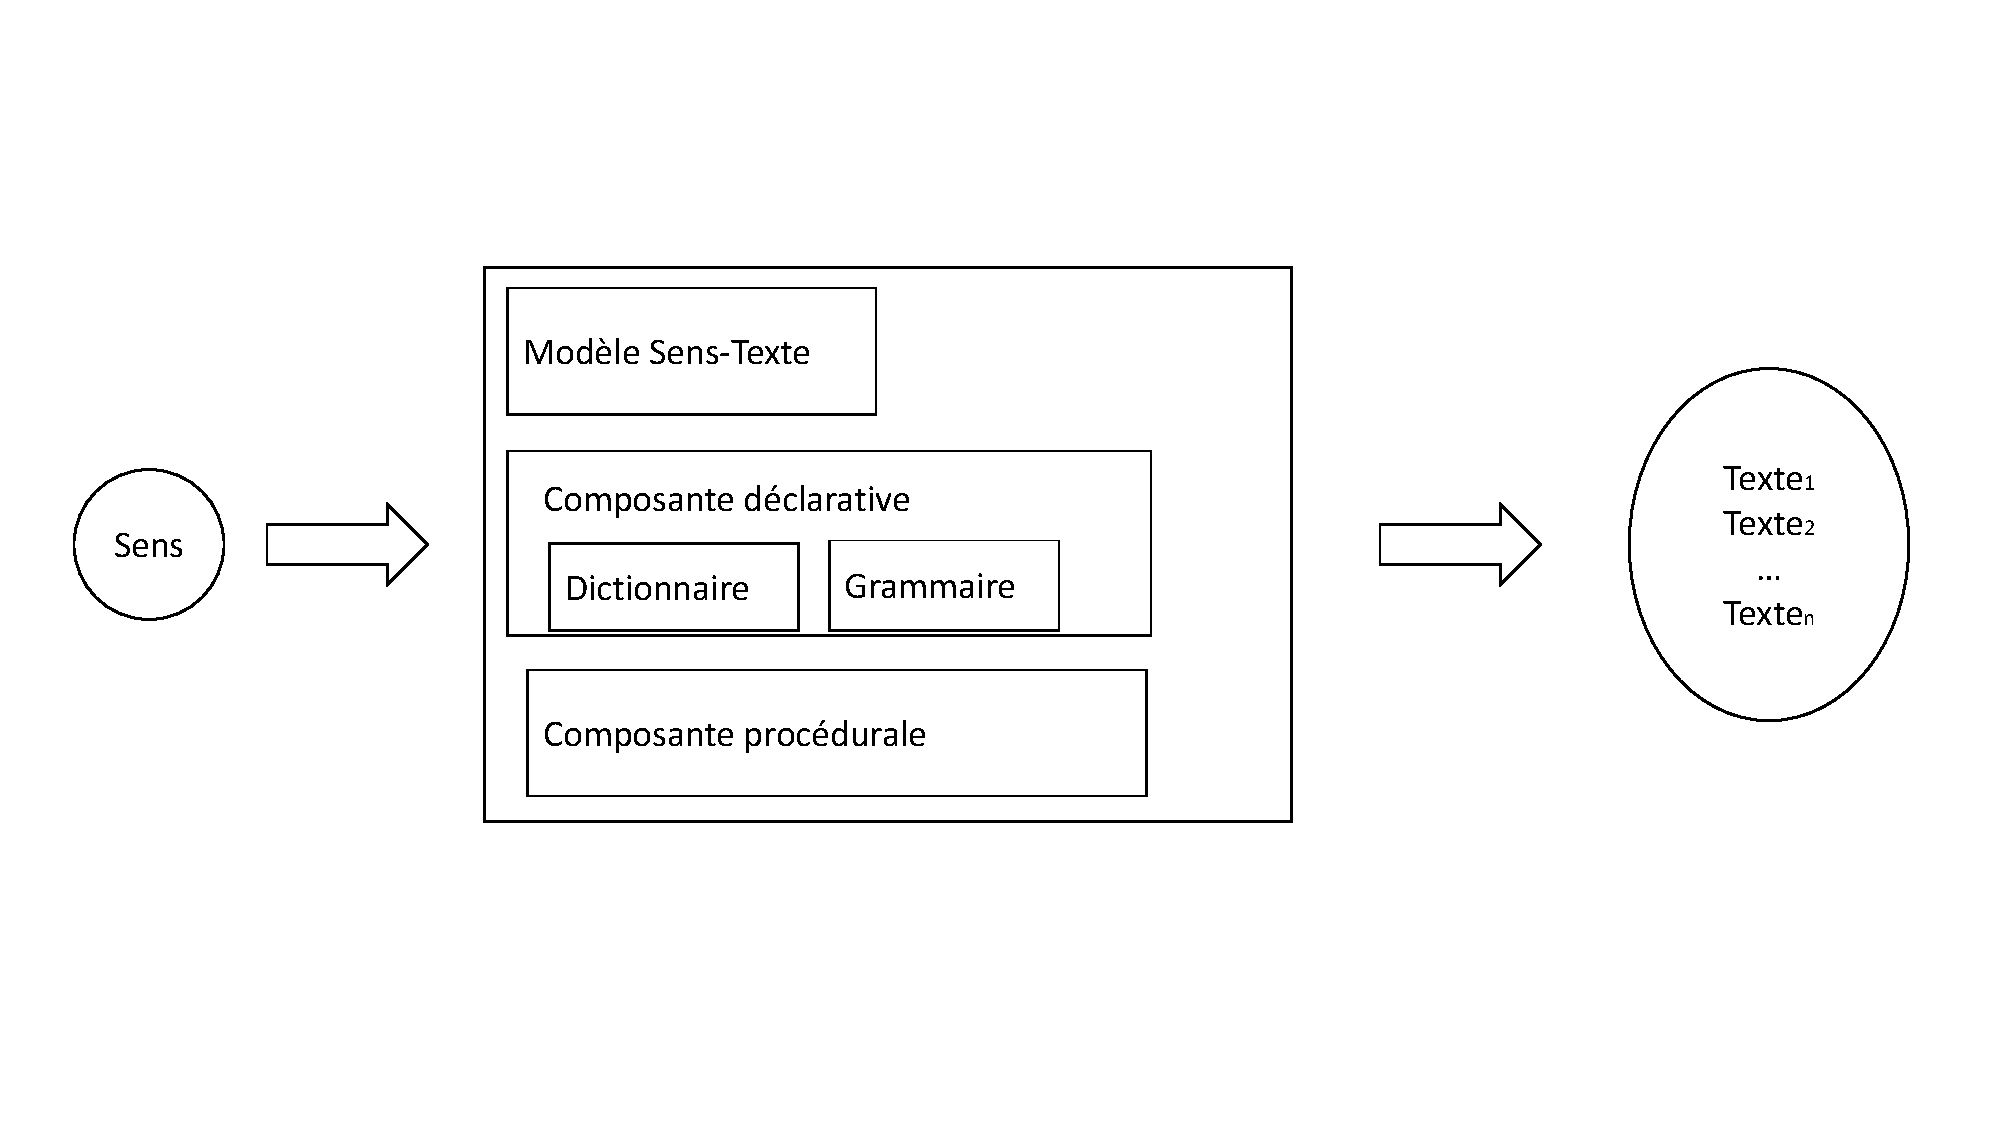
\includegraphics[width=1\textwidth, trim = {0cm 4cm 0cm 4cm},clip]{ch3/figs/polguere1.pdf}
	\caption{Structure d'un modèle Sens-Texte \citep{PolgueretheorieSensTexte1998}}
	\label{fig:modeletst}
\end{figure}

Pour se rendre au \emph{Texte} final, le \emph{Sens} traverse de nombreux niveaux de représentations. La figure \ref{fig:processustst} illustre les transformations que l'input doit subit succesivement. La figure illsutre aussi parallèlement le formalisme utilisé pour modéliser les représentations diverses.

\begin{figure}[htb]
	\centering
	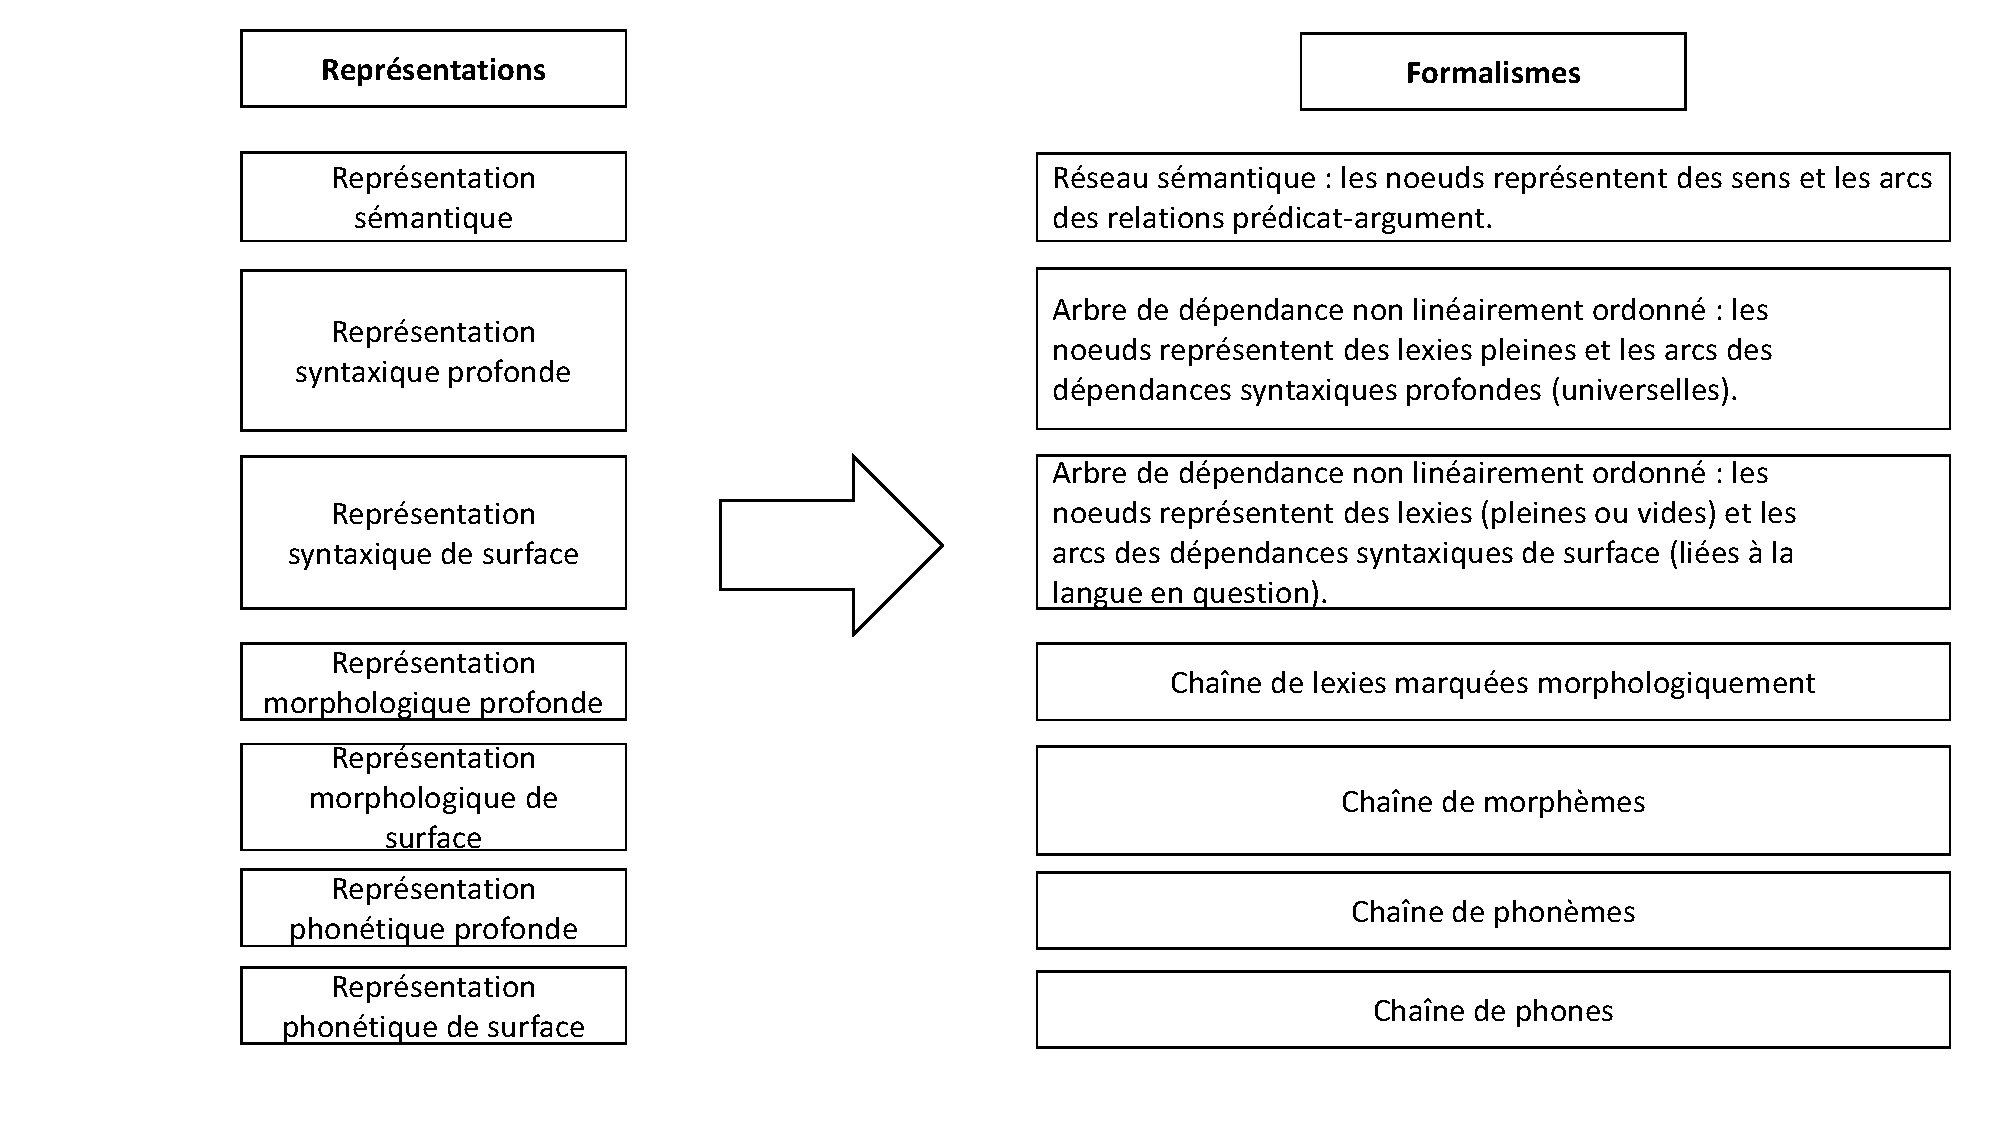
\includegraphics[width=1\textwidth, trim = {0cm 0cm 0cm 0cm},clip]{ch3/figs/polguere2.pdf}
	\caption{Processus d'un modèle Sens-Texte \citep{PolgueretheorieSensTexte1998}}
	\label{fig:processustst}
\end{figure}

%%%%%%%%%%%%%%%%%%%%%%%%%%%%%%%%%%%%%%%%%%%%
% --------- A R B O R I S A T I O N  ------
%%%%%%%%%%%%%%%%%%%%%%%%%%%%%%%%%%%%%%%%%%%

\subsection{Arborisation}\label{sec:arbo}

Tel que nous l'avons mentionné, le réalisateur GenDR modélise spécifiquement trois niveaux de représentations (\ac{RSem}-\ac{RSyntP}-\ac{RSyntS}). L'arborisation, qui est le processus de création de la syntaxe profonde à partir d'une structure sémantique, se situe dans ces trois niveaux. Nous la décrirons à la fois d'un point de vue théorique et comment cela se traduit dans le cadre de notre projet.

Selon la \ac{TST}, la structure syntaxique d'un énoncé représente l'ensemble des liens de dependances fonctionnelles qui existent entre les unités lexicales de cet énoncé \citep{melcuk1988}. On représente formellement ces structures syntaxiques par des arbres de dépendances. Cette approche syntaxique provient de \cite{TesniereElementssyntaxestructurale1965} qui est le premier à l'avoir théorisée. Formellement, le passage de la \ac{RSem} à la \ac{RSyntP} se nomme l'arborisation parce qu'on cherche à arboriser la structure sémantique pour qu'il en résulte un arbre de dépendance profond grâce à l'application de règles de correspondance sémantiques. Nous reprendrons donc la description que \cite{lareau18} fait de l'arborisation dans GenDR. D'ailleurs, l'arbre syntaxique profond est construit avec un algorithme \emph{top-down} qui ressemble énormément à celui qu'utilise FORGe puisque ces deux réalisateurs profonds l'ont hérité de MARQUIS, qui est inspiré de \cite{PolguereStructurationmisejeu1990}.

Bref, dans GenDR, l'arborisation se divise en trois étapes \citep{lareau18}.

\begin{enumerate}
  \item Création de la racine.
  La première règle appliquée est \emph{root\_standard}, elle construit la racine de l'arbre syntaxique à partir du \ac{ND} de la structure sémantique. À cette étape, la racine n'est pas étiquetée par un lexème encore (le n\oe{}ud est vide), mais des contraintes lui sont imposées. La détermination de la racine correspond au processus de hiérarchisation de \cite{PolguereStructurationmisejeu1990} car la racine est le n\oe{}ud dominant (au sommet de la hiérarchie) tous les autres.

  \item Lexicalisation de la racine.
  Une fois que la racine a été créée et contrainte, on applique une règle de lexicalisation (appellée \emph{lex\_standard}) qui permet au système de fouiller dans les dictionnaires pour trouver un lexème qui correspondra au sens demandé tout en respectant les contraintes imposées. Ainsi, il faut que le lexème sélectionné corresponde au \ac{ND} en sémantique et qu'il possède une \ac{DPOS} de type verbale généralement. Effectivement, les langues européennes imposent souvent cette contrainte sur la racine puisque ce sont essentiellement les verbes qui contrôlent les énoncés.

  \item Application des règles actancielles.
  Une fois que le n\oe{}ud racine est lexicalisé, GenDR regarde dans le \ac{GP} de la racine pour savoir comment effectuer le passage des arcs sémantiques aux arcs syntaxiques. Autrement dit, on ajoute les arcs dépendant de la racine qui correspondent aux arguments liés au \ac{ND} dans la \ac{RSem}. Comme Polguère le dit:
\begin{quote}
chaque arc est considéré successivement dans l'ordre du parcours, puis est traduit en une micro-structure syntaxique profonde grâce aux règles de correspondance sémantique de la grammaire.
\end{quote}
\vspace{-\baselineskip}
\hfill
\cite[p.~273]{PolguereStructurationmisejeu1990}

Les micro-structures syntaxiques correspondent aux branches de l'arbre et à leurs noe{}uds qui se font, à leur tour, imposer des contraintes par le \ac{GP} du noe{}ud qui les gouverne (la racine). C'est ainsi qu'on retourne à la seconde étape pour lexicaliser ces n\oe{}uds. Puis cycliquement, nous retournons à la troisième étape puisque de nouveaux n\oe{}uds lexicalisés amènent leur patron de régime avec eux. Et ce jusqu'à ce que le graphe sémantique soit complètement réalisé en surface profonde.
\end{enumerate} 

Une fois que l'arborisation est complétée, le système doit effectuer l'arborisation de surface ce qui implique les opérations suivantes. D'abord, faire le calcul des relations syntaxiques de surface (la relation I deviendra sujet, la relation II deviendra complément d'objet direct, etc.) et incorporer les lexies vides (prépositions, déterminants, etc.). Cela est effectué grâce aux règles de correspondances profondes et aux informations contenues dans les \ac{GP} des entrées lexicales.

%%%%%%%%%%%%%%%%%%%%%%%%%%%%%%%%%%%%%%%%%%%%%%%%%%%%%
% ---------  L E X I C A L I S A T I O N  ------
%%%%%%%%%%%%%%%%%%%%%%%%%%%%%%%%%%%%%%%%%%%%%%%%%%%%
\subsection{Lexicalisation}

Le processus de lexicalisation est dispersée sur plusieurs niveaux de représentation (\ac{RSem}, \ac{RSyntP}, \ac{RSyntS}) formant deux interface (\ac{RSem}-\ac{RSyntP}, \ac{RSyntP}-\ac{RSyntS}) \citep{PolguerePourmodelestratifie}. La première interface modélise la lexicalisation profonde qui consiste à assure la correspondance entre une unité sémantique dont les traits \texttt{definiteness} ou \texttt{tense} (voir figure \ref{fig:debt}) sont remplacés par des traits grammaticaux et dont le sens est remplacé par une (ou des) unité(s) lexicale(s) profonde(s). Cette correspondance est explicité dans le dictionnaire d'un système \ac{TST}. S'ensuit la lexicalisation de surface qui consiste à introduire les mots fonctionnels (déterminants, auxiliaires, prépositions,etc.) et les lexies de surface (comme dans l'exemle que nous avons montré plus haut avec peur bleu où bleu serait réalisée en surface). \draft{Daniel: Je n'ai pas trouvé la citation sur la lexicalisation de Wanner dont tu parlais (dans le mémoire de Flo)}

Afin d'illustrer le fonctionnement de la lexicalisation dans GenDR, nous repredrons la description de \cite{lareau18}.

\textbf{Les lexicalisations simples}
sont traitées par la règle \emph{lexicalization\_standard} qui prend une unité sémantique donnée dans un graphe d'input et récupères dans le \emph{semanticon} les correspondances lexicales de ce sémantème (tel que démontré en \ref{fig:semanticon}). S'ensuit la sélection de l'unité lexicale: GenDR s'assure que la \ac{DPOS} de la (ou les) lexie(s) correspond à celle qui est demandée par le n\oe{}ud contraint dans l'arbre syntaxique profond en construction. Le no\oe{}ud en question de l'arbre syntaxique profond sera désormais lexicalisé. D'ailleurs, c'est ce mécanisme qui permet le paraphrasage dans notre système, puisqu'il crée autant d'arbres syntaxiques profonds qu'il y a de lexies possibles pour un n\oe{}ud donné.

\textbf{Les lexicalisations de classes}
comme les nombres, les montants, les noms propres ou les acronymes sont prises en charge par la règle \emph{lex\_class}. Sont but est de lexicaliser les unités sémantiques que nous ne voulons pas dans nos dictionnaires sémantiques et lexicaux parce qu'elles sont trop nombreuses et leur comportement est prévisible. Pour déclencher l'application de cette règle, on précise dans la structure d'input à quelle classe le sémantème appartient. Celle-ci contient les informations nécessaires à la lexicalisation d'un n\oe{}ud donné (la \ac{DPOS}, la \ac{SPOS}, le nombre, l'invariabilité, la comptabilité,etc.)

\textbf{La lexicalisation de secours} 
permet à GenDR de lexicaliser une unité sémantique ou lexicale dont il n'a pas les informations. Effectivement, comme le système possède les 1\,500 lexies les plus fréquentes de l'anglais, il est évident que certaines lexies ou sémantèmes manqueront à l'appel. Pour remédier à la situation, il y a d'abord un mécanisme qui vérifie si l'input existe sous la même forme dans le \emph{lexicon}. Si c'est le cas, alors le système réalisera le sémantème à l'aide de ce lexème. Cette particularité du système a pour conséquence qu'on n'a pas besoin d'inscrire le sémantème dans le \emph{semanticon} s'il n'y a qu'une seule lexicalisation possible de celui-ci (cela permet de sauver du temps). Cependant, si le sémantème ne figure pas dans le \emph{lexicon}, alors le système suppose que l'étiquette de l'unité sémantique est la même que l'unité lexicale, et s'il y a des contraintes sur le n\oe{}ud d'arrivée, alors le système supposera que l'unité lexicale ainsi créée satisfait les contraintes. Les lexèmes devinés seront mis en évidence dans la structure d'output afin qu'on ait une trace que le système a fait une tentative.

\textbf{La lexicalisation grammaticale}
introduit des lexèmes fonctionnels (dét., aux., etc.) et prend place au entre la \ac{RSyntP}-\ac{RSyntS}. Ce type de règle est déclenché par la présence de sens grammaticaux dans les structures d'input comme la définitude ou le temps (voir la figure \ref{fig:debt}). Ces lexèmes existent en syntaxe profonde, mais sous forme de traits sur les n\oe{}uds lexicaux. Comme ces lexies appartiennent à une classe fermée et qu'ils sont peu nombreux (en plus d'être spécifiques à une langue), ils sont lexicalisés par une règle spéciale qui sait comment réaliser les traits grammaticaux. Puis, il y a aussi des règles de lexicalisation grammaticales qui s'occupent des lexèmes imposés en surface par les régimes de certaines lexies (comme les prépositions). Ce type de lexème est introduit en syntaxe comme un n\oe{}ud supplémentaire entre un gouverneur et son actant. Ils sont donc encodés dans le \ac{GP} du gouverneur. \draft{pas clair}

%%%%%%%%%%%%%%%%%%%%%%%%%%%%%%%%%%%%%
% --------- E X E M P L E ---------
%%%%%%%%%%%%%%%%%%%%%%%%%%%%%%%%%%%%%

\section{Exemple}\label{sec:exemple}

Pour illustrer le fonctionnement des règles et des dictionnaires que nous venons de présenter, nous décortiquerons la réalisation profonde de l'exemple vu à la figure~\ref{fig:debt}.

\subsection{Arborisation profonde}

Cette section illustre les étapes successives qui ont permis à GenDR de passer de la \ac{RSem} à la \ac{RSyntP}.

\subsubsection{Application de la règle \emph{root\_standard}}
La règle crée un n\oe{}ud vide qui sera la racine de l'arbre à construire et qui se fait imposer les contraintes suivantes: \texttt{dpos=V} (la racine doit être un verbe) et \texttt{finiteness=FIN} (tensé). La figure \ref{fig:rootstand} illustre la création du n\oe{}ud non-étiqueté.
\begin{figure}[htb]
	\centering
	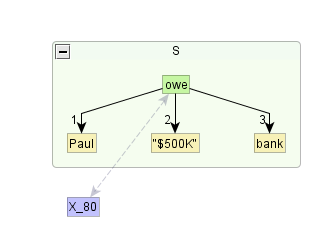
\includegraphics[width=0.6\textwidth, trim = {1cm 0.5cm 0cm 1cm},clip]{ch3/figs/inspecteur_root.png}
	\vspace{-0.5cm}
	\caption{Application de \emph{root\_standard}}
	\label{fig:rootstand}
\end{figure}

\subsubsection{Application de la règle \emph{lex\_standard}}
La racine vide déclenchera l'application d'une règle de lexicalisation, c'est pourquoi GenDR fouillera dans le dictionnaire à la recherche des lexèmes représentant le sémantème \sem{owe} \lstinline! owe { lex=owe lex=debt}!. GenDR peut ainsi lexicaliser la racine en choisissant \lex{debt} ce qui entraînera l'application d'une fonction lexicale permettant de réaliser un verbe support à la racine (ce qui satisfait la contrainte \texttt{dpos=V}). Il s'agit d'une lexicalisation complexe, donc nous renvoyons le lecteur à \cite{lambrey15,LambreyImplementationcollocationspour2017,lareau18} pour nous concentrer sur la lexicalisation simple effectuée grâe au lexème \lex{owe}.

\begin{figure}[htb]
	\centering
	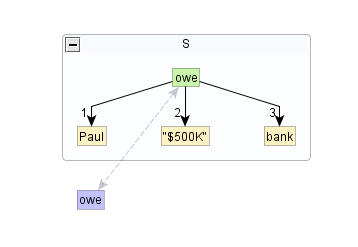
\includegraphics[width=0.7\textwidth, trim = {0cm 0.7cm 0cm 0.9cm},clip]{ch3/figs/lex_standard_root.png}
		\vspace{-0.5cm}
	\caption{Application de lex\_standard}
	\label{fig:lexstand1}
\end{figure}

\subsubsection{Application de la règle \emph{actant\_gp}}
Une fois que la racine est pourvue d'un lexème, l'application de la règle \emph{actant\_gp} est déclenchée. Celle-ci traduit les relations sémantique prédicat-argument de \sem{owe} en arcs syntaxiques profonds. La correspondance est confirmée par les informations sur la diathèse encodée dans le régime de la lexie \lex{owe}. Comme le prédicat lie trois actants sémantiques, alors la règle s'applique trois fois pour chaque relation. Ensuite, les n\oe{}uds au bout des arcs syntaxiques seront contraints en fonction des restrictions prévues par le \ac{GP} de \lex{owe}. Ce mécanisme assure la grammaticalité de la construction de l'arbre. Pour cet exemple, le \ac{GP} de \lex{owe} permet à son deuxième actant syntaxique d'être soit un nom ou un nombre (la figure \ref{fig:dictio} illustre le régime du verbe).

\begin{figure}[htb]
	\centering
	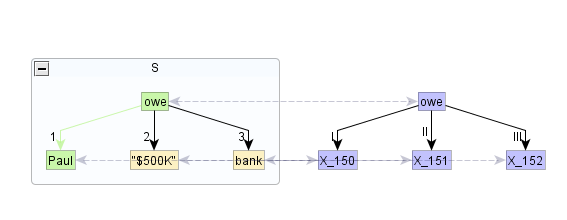
\includegraphics[width=1\textwidth, trim = {0cm 8mm 0cm 15mm},clip]{ch3/figs/actant_gp1.png}
	\caption{Application de actant\_gp}
	\label{fig:actantgp}
\end{figure}

\subsubsection{Application des règles \emph{lex\_class} et \emph{lex\_standard}}

L'étape précédente a généré des arcs contraints en partance de la racine. Les n\oe{}uds de ces arcs devront donc être lexicalisé afin de poursuivre l'arborisation. GenDR répètera opèrera deux règles de lexicalisation pour ce faire afin de réaliser les lexèmes correspondant à \sem{Paul}, \sem{bank} et \sem{\$500}. Les règles (\emph{lex\_class}) et (\emph{lex\_standard}) seront utilisés puisque \sem{Paul} et \sem{\$500} affichaient les traits respectifs \texttt{class=proper\_noun} et \texttt{class=amount} dans l'input sémantique. La règle fait en sorte que GenDR passe directement au \emph{lexicon}, puisque les sens ne sont pas décrits dans le \emph{semanticon}. L'étiquette du n\oe{}ud sémantique est directement copiée en syntaxe puis GenDR s'assure finalement que les traits de \lex{Paul} et \lex{\$500} respectent les contraintes des n\oe{}uds générés par la règle précédente.

\begin{figure}[htb]
	\centering
	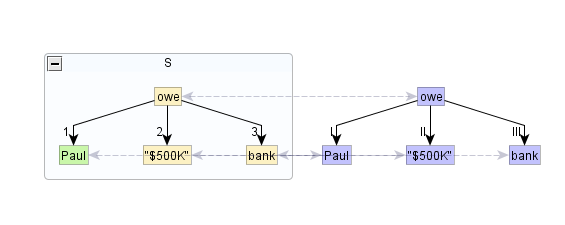
\includegraphics[width=1\textwidth, trim = {0cm 8mm 0cm 10mm},clip]{ch3/figs/lex_standard2.png}
	\caption{Application des règles de lexicalisation}
	\label{fig:lexstand2}
\end{figure}

\FL{trim les figures}

\subsection{Arborisation de surface}

\subsubsection{Application des règles de lexicalisation de surface}
On va chercher les lexicalisations de surface de chacune des unités lexicales avec les règles \emph{lex\_class} (qui s'occupe des lexèmes comme \lex{Paul}) et \emph{lex\_lu}. Il y en a deux, car il faut une règle spécifique pour les lexèmes appertenant à des classes puisque leurs traits de surface ne sont pas encodé dans leurs entrées lexicale, mais dans la classe qui leur est assignée.

\begin{figure}[htb]
	\centering
	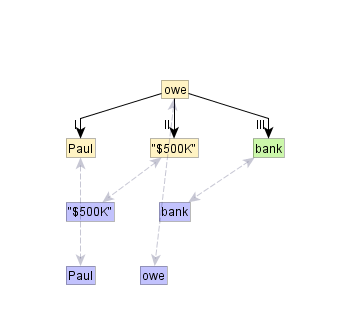
\includegraphics[width=0.6\textwidth, trim = {0cm 13mm 0cm 2cm},clip]{ch3/figs/rsyntslexicalisation1.png}
	\caption{Application des règles de lexicalisation de surface}
	\label{fig:lexsurf}
\end{figure}

\subsubsection{Application des règles actancielles de surface}
Concrètement, ces règles remplacent les étiquettes des branches de l'arbre profond (I, II, III,...) par des étiquettes de surface (sujet, objet direct, objet indirect,...) qui sont encodées dans le \ac{GP} du gouverneur. Ainsi, il y a une règle pour la relation subjectale (actant\_subj), la relation objective directe (actant\_obj) et les relations indirectes/obliques nécessitant des prépositions en surface (\emph{actant\_prep}). Par exemple, le \ac{GP} du gouverneur contient l'information suivante pour réaliser le sujet: \lstinline!gp = { I = { dpos = N \textbf{rel = subjective} } } !.

La règle \emph{actant\_prep} diffère des deux autres règles actancielles car elle crée un n\oe{}ud intermédiaire en syntaxe de surface permettant d'accueillir le lexème fonctionnel \lex{to} qui est nécessaire à la bonne formation de la phrase. La préposition est directement encodée dans le \ac{GP} du verbe: \lstinline! gp = {III = { dpos = N  rel = indir_objective  \textbf{prep = to} }  }!.

\subsubsection{Application de la règle des déterminants}

La règle \emph{det\_def} ajoute les déterminants aux lexèmes en fonction de leur définitude. Parmi les règles que nous avons présenté, c'est la seule règle de GenDR qui est propre à l'anglais. Dans l'exemple présent, elle lexicalise \lex{the} puisque l'unité sémantique \sem{bank} était marquée par le trait défini dans la structure d'input.

La figure \ref{fig:syntsurf} démontre l'application des règles actancielles et de la règle des déterminants.

\begin{figure}[htb]
	\centering
	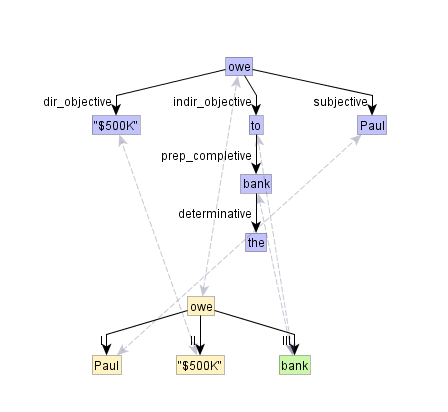
\includegraphics[width=0.7\textwidth, trim = {0cm 8mm 0cm 15mm},clip]{ch3/figs/rsynts_syntactisation.png}
	\caption{Application des règles actancielles de surface et des déterminants}
	\label{fig:syntsurf}
\end{figure}

%%%%%%%%%%%%%%%%%%%%%%%%%%%%%%%%%%%%%%%%%%%%%%%%
% --------- P R O B L É M A T I Q U E ---------
%%%%%%%%%%%%%%%%%%%%%%%%%%%%%%%%%%%%%%%%%%%%%%%%

\section{Problématique}\label{sec:problema}

\draft{à relire}

La démonstration précédente montre que GenDR modélise avec aisance des phénomènes linguistiques profonds. Toutefois, le dictionnaire lexical de ce système ne couvre que les 1\,500 lexies les plus fréquentes (en anglais et en français) dont 500 sont des verbes. Cela est non-négligeable, certes, mais il est clair que GenDR gagnerait en couverture s'il se dotait d'une ressource lexicale lui permettant de traiter une plus grande quantité de verbes. Pourquoi les verbes en particulier ? Parce que les verbes contrôlent la plupart des énoncés et ils démontrent des irrégularités quant à leur comportement syntaxique. Donc, en détenant les propriétés lexicales de combinatoire des verbes d'une langue donnée, on peut couvrir une immense partie de celle-ci

\begin{quote}
In particular, since verbs often convey the main idea of a sentence, such a resource must represent verb meanings. These require a particularly precise and well deffined representation that captures both their predicate-argument structure as well as their semantic content.
\end{quote}
\vspace{-\baselineskip}
\hfill
\cite{SchulerVerbnetBroadcoverageComprehensive2005}

Nous sommes en accord avec cette déclaration, tout comme \cite{Korhonenlargesubcategorizationlexicon2006} qui suggèrent aussi que la modélisation informatique des langues naturelles passe par de telles ressources lexicales (dictionnaire de cadres de sous-catégorisation).  Notre objectif est d'intégrer, au réalisateur profond GenDR, un dictionnaire doté des \acp{GP} des verbes de la langue anglaise.

\section{Patrons de régime}\label{sec:gp}

D'abord, il faut préciser que ce qu'on appelle \ac{GP} se nomme de différentes manières selon le cadre théorique utilisé: cadre valenciel, valence, cadre de sous-catégorisation, cadre syntaxique ou schéma de régime. Selon \cite{MilicevicSchemaregimepont2009}, les \acp{GP} décrivent les cooccurrences syntaxiques des unités lexicales avec leurs actants (les sujets et objets des verbes, les compléments du nom,etc.). Autrement dit, les \acp{GP} d'une lexie correspondent à l'ensemble des constructions syntaxiques dont la lexie est la gouverneure. On les encode dans un dictionnaire car les \acp{GP} des lexies ne sont généralement pas prévisibles (le nombre d'actant, la diathèse, la préposition qu'un actant sélectionne, le fait de pouvoir sélectionné des unités appartenant à une seule partie du discours ou plusieurs, etc.). D'ailleurs, même des verbes sémantiquement proches ne possèderont pas nécessairement les mêmes constructions syntaxiques, ce qui est illustré par \cite{MilicevicSchemaregimepont2009}: \form{on se souvient de X }, mais \form{on se rappelle X}.

Plus tôt dans le chapitre, nous avions parlé de l'interface sémantique-syntaxe et de l'importance des règles de correspondance sémantiques qui font la transition entre \ac{RSem} et \ac{RSyntP}. Le rôle le plus important du \ac{GP} est de fournir l'information nécessaire au passage de la \ac{RSem} à la \ac{RSyntP} lors des opérations de lexicalisation et d’arborisation. Le patron de régime d'une lexie encode les correspondances entre ses actants (au niveau sémantique, syntaxique profond et syntaxique de surface), les moyens morpho-syntaxiques d'expressions des actants et les restriction sur les actants (ex: \texttt{dpos=N}). Les \acp{GP} encodent la diathèse qui est la correspondance entre les actants sémantiques d'une lexie et ses actants syntaxiques profonds. Celle-ci peut soit être triviale (\texttt{1=I,2=II,3=III}) ou pas (\texttt{1=I, 2=III, 3=II}) sans que cela n'affecte le sens de l'énoncé. Il s'agit seulement d'une réorganisation des actants lors de l'arborisation. Le \ac{GP} encore aussi la réalisation des actants en surface (\texttt{I=sujet, II= objet direct}, etc.).

\begin{quote}
Comme le choix lexical détermine le choix des constructions syntaxiques possibles (la lexie sélectionnée « amène » avec elle son régime) et vice-versa (le choix d’une structure impose certains choix lexicaux), on peut dire que c’est le schéma de régime qui, au sein d’un MST\draft{est-ce que je précise que ça veut dire Modèle Sens-Texte ?}, fait le pont entre le lexique et la grammaire.
\end{quote}
\vspace{-\baselineskip}
\hfill
\cite[p.~105]{MilicevicSchemaregimepont2009}

L'une des raisons qui nous a poussé à nous retourner vers une ressource lexicale verbale provient des limites du logicel MATE \citep{BohnetDevelopmentEnvironmentMTTbased2000,BOHNET10,bohnet07} que nous utilisons. Ce logiciel présente des limites quant à l'encodage de multiples patrons de régime pour une même entrée.

Pour un verbe donné, on ne peut pas avoir deux parties du discours différentes qui compétitionnent pour la même position syntaxique. Autrement dit, si nous voulions exhaustivement représenter les comportements du verbe \lex{want}, il nous faudrait un \ac{GP} qui puisse tenir compte du fait que le second actant syntaxique de ce verbe peut avoir une \ac{DPOS}de type verbale ou nominale: \form{I want to eat.} vs \form{I want a dog.}. Cela nous était impossible à encoder dans MATE avec les paramètres que nous avions car le système ne nous laissait pas donner deux version de l'actant syntaxique II de \lex{want}. Ce qui s'offrait à nous comme solution était de créer deux verbes \lex{want} qui encoderaient séparés ces comportements syntaxiques. Nous étions conscients que ce n'était pas viable et il nous fallait trouver une solution à ce problème. Nous nous sommes alors retourné vers l'idée d'ajouter un dictionnaire supplémentaire à notre ressource, qui encoderait tous les régimes existant de l'anglais. Puis, nous n'aurions qu'à encoder l'identification des \ac{GP} dans les unités lexicales appropriées ce qui nous permettait de contourner le problème des \acp{GP} multiples.

Notre ancienne méthode restreignait conséquemment le nombre de génération possible pour un verbe donné ou peuplait inutilement le dictionnaire d'entrées verbales en fonction des diverses restrictions sur les actants syntaxiques.

De plus, en allant chercher une ressource comme celles qui rassemble les patrons de régime des verbes, nous allons aussi chercher les verbes. Donc nous enrichissons le contenu lexical de notre dictionnaire en plus de trouver une solution au problème. Afin d'augmenter notre couverture, il aurait fallu manuellement enregistrer les verbes de l'anglais et c'est une tâche qui aurait pris énormément de temps. Ainsi, plusieurs groupes de recherches ont travaillé pour bâtir des ressources lexicales riches en comportements syntaxiques afin que les applications \ac{TAL} en bénéficient.
